\documentclass{beamer}

\usepackage[utf8]{inputenc}

\title{Logistiksystem für einen Veranstaltungsbetrieb}
\author{Niklas Arnitz\\WHG-Durmersheim}

\begin{document}

\begin{frame}
	\maketitle
\end{frame}

\begin{frame}
	\tableofcontents
\end{frame}

\section{Anforderungsanalyse}
\begin{frame}
	\frametitle{Anforderungsanalyse}
	
	\begin{itemize}
		\item Mehrere Nutzer sollten das System unabhängig voneinander nutzen können
		\item Es sollen Artikel vermietbar/ausleihbar sein
		\item Es soll eine Übersicht geben, welcher Artikel gerade wo ist
		\item Es sollte ein komplettes Inventar angelegt werden können
	\end{itemize}
\end{frame}

\section{Aufbau der Applikation}
\begin{frame}
	\frametitle{Aufbau der Applikation}
	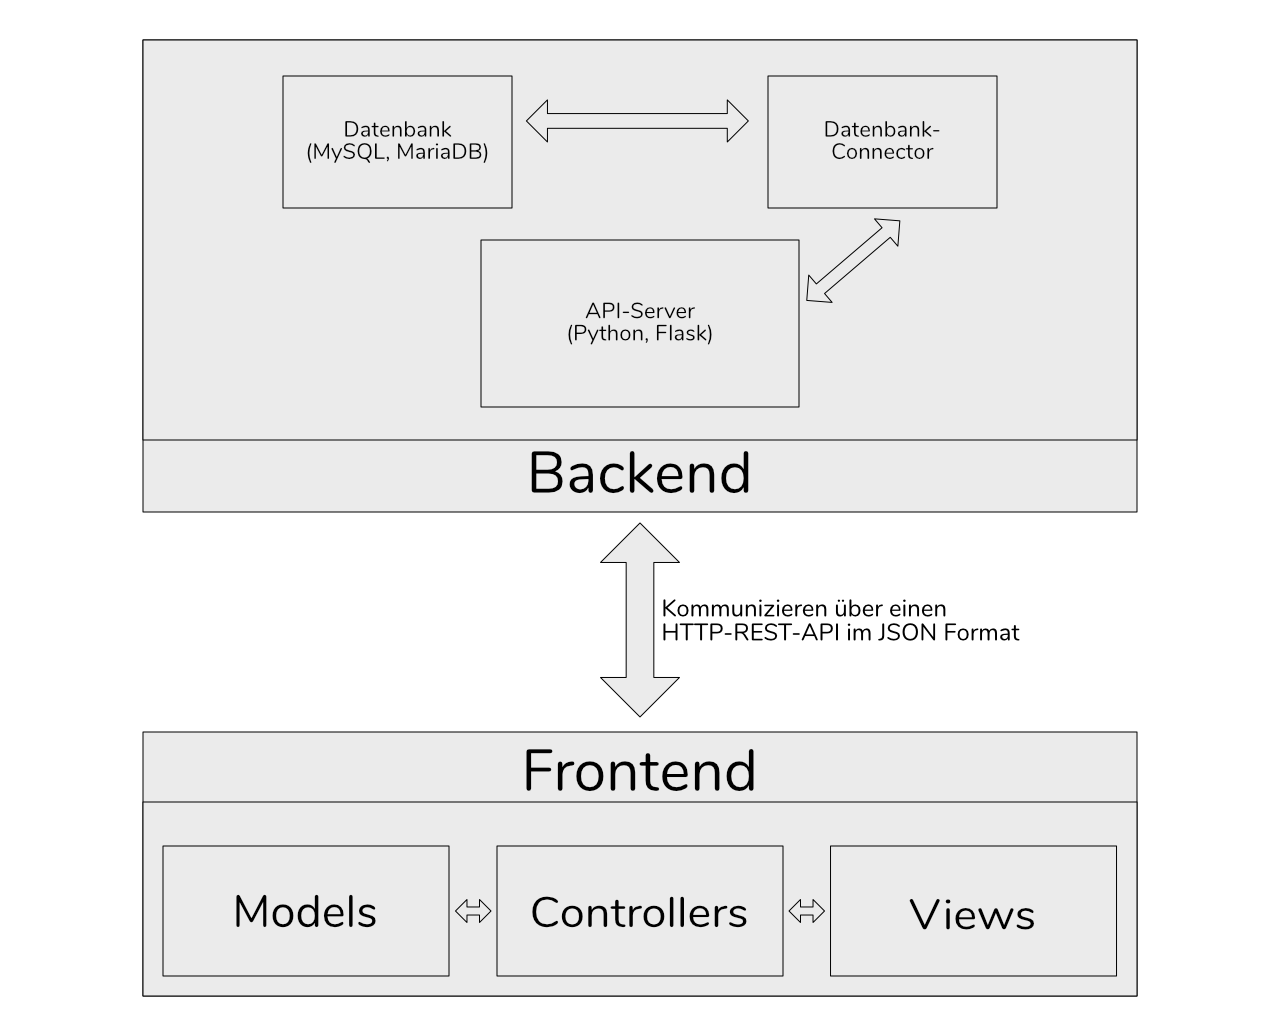
\includegraphics[width=\textwidth]{01-logistiksystem-aufbau}
\end{frame}

\section{ER-Diagramm}
\begin{frame}
	\frametitle{ER-Diagramm}
\end{frame}

\section{Implementierung des ER-Diagramms}
\begin{frame}
	\frametitle{GUI/Webinterface}
\end{frame}

\end{document}
